\section{Privacy-Preserving Edit Distance Computation}
\label{sec:protocols}

\subsection{Edit distance: definition}
\label{sec:edit-distance}

Let $\alpha$ and $\beta$ be two strings over an alphabet $\Sigma$.
Let the lengths of the two strings $\alpha$ and $\beta$ (denoted by $ \mid
\alpha \mid $ and $ \mid \beta \mid $) be $n$ and $m$, respectively. The
edit-distance between the two strings $\alpha$ and $\beta$ (denoted by
$\delta (\alpha,\beta)$) is the minimum number of edit operations ({\sf
delete}, {\sf insert}, and {\sf replace}) needed to transform $\alpha$
into $\beta$.  The following dynamic programming algorithm computes
$\delta (\alpha,\beta)$ in time $O(nm)$~\cite{Gusfield}.

Given a string $\alpha$, let $\alpha [1 \cdots i]$ denote the first $i$
characters of $\alpha$.  The dynamic programming algorithm maintains a
$(n+1) \times (m+1)$ matrix $D(0 \cdots n, 0 \cdots m)$, where $D(i,j)$ is
the edit distance between $\alpha [1 \cdots i]$ and $\beta [1 \cdots j]$.

For the base case, we have the following:
\begin{eqnarray}
\label{eqn:base-case}
D(i,0) & = & i \;\; , \; 0 \leq i \leq n \\
D(0,j) & = & j \;\; , \; 0 \leq j \leq m
\end{eqnarray}
Next we describe a recursive relationship between the value $D(i,j)$ 
and the entries of $D$ with indices smaller than $i$ and $j$.
The $(i,j)$-th entry $D(i,j)$ of the matrix is computed as follows:
\begin{eqnarray}
\label{eqn:recursive}
D(i,j) & = & \mbox{min} [ D(i-1,j) + 1, D(i,j-1)+1,  D(i-1,j-1)+t(i,j) ] 
\end{eqnarray}
where $t(i,j)$ is defined to have value $1$ if $\alpha (i) \not= \beta
(j)$, and has value $0$ if $\alpha (i) = \beta (j)$. The $i$-th character
of a string $\alpha$ is denoted by $\alpha (i)$. The entire algorithm for
computing edit distance is shown in Figure~\ref{fig:edit-distance-alg}.

\begin{figure}
\framebox{\parbox[c]{6.2in}{
\begin{itemize}

\item Compute $D(i,0)$ and $D(0,j)$ for $1 \leq i \leq n$ and $1 \leq j \leq m$ using
equation~\ref{eqn:base-case}.

\item Compute $D(i,j)$ for $1 \leq i \leq n$ and $1 \leq j \leq m$ in row major order
using equation~\ref{eqn:recursive}. In other words, we first compute all entries for
row $1$, then row $2$, and so on.

\item The edit distance $\delta(\alpha,\beta)$ is equal to $D(n,m)$.
\end{itemize}
}}
\caption{Algorithm for computing edit distance.}
\label{fig:edit-distance-alg}
\end{figure}


\subsection{Preserving privacy in edit distance computation}

In the rest of this section, we will consider Alice ($A$) and
Bob ($B$), who want to use the dynamic programming algorithm
of section~\ref{sec:edit-distance} to compute the edit distance
$\delta(\alpha,\beta)$ between their respective strings $\alpha$
(of size $n$) and $\beta$ (of size $m$), but do not want to reveal
the strings themselves.  For example, ``Alice'' and ``Bob'' could be
medical institutions participating in an NIH-sponsored collaborative
study, while the strings in questions could be genome sequences with
significant intellectual-property value.

We present three protocols.  Protocol 1 is the ``base case,'' representing
straightforward application of generic techniques.  Protocol 2 uses
very small circuits in combination with the SWCS protocol.  Protocol 3
exploits the fundamental structure of the dynamic programming problem.
It divides the matrix $D$ into a grid and uses it to split the
instance into subproblems of size $(k,k)$, where $k$ divides both $n$
and $m$.  The differences between the protocols are summarized in
Figure~\ref{fig:protocol-characteristics}.

\begin{figure}
\begin{center}
\begin{tabular}{|c|c|c|c|} \hline
 {\sf\small Number of Iterations} & {\sf\small Round complexity} & 
{\sf\small Optimized round complexity} & {\sf\small  Circuits used} \\ \hline
Protocol 1 & $1$ & 1 & Circuit for \\ 
(generic)  & & & $(n,m)$ instance \\ \hline
Protocol 2 & $O(nm)$  & $O(m+n)$ & Circuits for \\
	   & & & equality testing and \\
           & & & ``minimum-of-three'' \\ \hline
Protocol 3 & $O(\frac{nm}{k^2})$  & $O(\frac{m+n}{k})$ & Circuit for \\ 
           & & &  $(k,k)$ instance \\ \hline
\end{tabular}
\end{center}
\caption{Characteristics of various protocols for problem of size $(n,m)$.}
\label{fig:protocol-characteristics}
\end{figure}

\subsection{Protocol 1}

Recall that the edit-distance algorithm maintains a $(n+1) \times
(m+1)$ matrix $D(0 \cdots n, 0 \cdots m)$, where $D(i,j)$ is the
edit distance between $\alpha [1 \cdots i]$ and $\beta [1 \cdots j]$.
Strings $\alpha$ and $\beta$ can be expressed as bit strings ${\it
bit}(\alpha)$ and ${\it bit}(\beta)$ of length $qn$ and $qm$, where $q$
is equal to $\lceil \log_2 (\mid \Sigma \mid) \rceil$.

The base case and recursive equation for computing $D(i,j)$ were given
in equation~\ref{eqn:base-case}. Let $C_{D(i,j)}$ be the circuit for
computing $D(i,j)$ with inputs corresponding to bit representation of
$\alpha [1,\cdots,i]$ and $\beta [1,\cdots,j]$. Assume that we have
computed $C_{D(i-i,j)}$, $C_{D(i,j-1)}$, and $C_{D(i-1,j-1)}$. The
recursive computation given by equation~\ref{eqn:recursive} can be
represented as a circuit $C_{D(i,j)}$, which computes $D(i,j)$ by
combining (i) the equality testing circuit for $t(i,j)$, (ii) three
``add-1'' circuits, and (iii) two ``select-smaller-value'' circuits.

The inputs to the circuit $C_{D(i,j)}$ are bit representations of
$\alpha[1,\cdots,i]$, $\beta[1,\cdots,j]$ and the outputs of circuits
$C_{D(i,j-1)}$, $C_{D(i-1,j)}$, and, $C_{D(i-1,j-1)}$.  Once we have
the circuit representation $C_{D(n,m)}$ for the edit distance problem,
we can compute $C_{D(n,m)}(\alpha,\beta)$ in a privacy-preserving
manner using standard algorithms for secure circuit evaluation (see
section~\ref{crypto}).


\subsection{Protocol 2}

Protocol 1 represents the entire problem instance as a single circuit.
The resulting representation, however, is impractically large for
problems of realistic size (see section~\ref{sec:experimental}).
Protocol 2 is designed to use much smaller circuits as building blocks.
It employs Yao's ``garbled circuits'' technique for circuit evaluation
in a non-black-box way, \ie, it exploits the \emph{specific circuit
representation} in Yao's protocol instead of using it simply as an
``ideal functionality'' for secure circuit evaluation.

Let $w=\mid \Sigma \mid$ be the size of the alphabet for which the two
strings are drawn, and recall that $q = \lceil \log_2 (w) \rceil$.
Let $r$ be the length of wire keys in Yao's ``garbled circuits''
construction (see section~\ref{yao}); $r$ can be viewed as the security
parameter for Yao's protocol.  Protocol 2 involves evaluation of multiple
instances of the following two circuits.

\newcommand{\CE}{C_{\mathit{eq}}}
\newcommand{\CM}{C_{\mathit{min3}}}

\vspace{1ex}
\noindent
\textbf{Equality testing circuit.}
Circuit $\CE$ is the standard logic circuit for testing equality of
two values.  Its inputs are two $q$-bit values, $x$ from Alice and $y$
from Bob.  The output for Alice is empty, and the output for Bob is
supposed to be the outcome of the comparison, \ie, $0$ if $x=y$, and $1$
if $x \neq y$. $\CE$ is a standard circuit consisting of $2q-1$ gates.

Recall that in Yao's construction, the circuit creator generates
two random $r$-bit ``wire keys'' for each circuit wire, including the
output wire.  Let $k^0_{\mathit{eq}}$ (respectively, $k^1_{\mathit{eq}}$)
be the wire key representing $0$ (respectively, $1$) on the output wire
of circuit $\CE$.  In our protocol, we will assume that the output of
$\CE$ is not the bit $\sigma$, which is the result of the comparison,
but instead the $r$-bit random value $k^{\sigma}_{\mathit{eq}}$, which
\emph{represents} $\sigma$.  Observe that this is \emph{not} a black-box
use of the ``ideal two-party computation functionality,'' because it
critically depends on the internal representation of circuit outputs
by random wire keys.  (In other words, an alternative implementation of
the same functionality would not be sufficient for our purposes.)

Bob, acting as the circuit evaluator in Yao's protocol, learns
$k^{\sigma}_{\mathit{eq}}$.  He does not learn whether this value
represents $0$ or $1$, since he does not know the mapping from random
wire keys to the bit values they represent (see section~\ref{yao}).
This property, too, is essential in our construction.

\vspace{1ex}
\noindent
\textbf{Minimum-of-three circuit.}
Circuit $\CM$ computes the minimum of three values, each of which is
randomly shared between Alice and Bob, and splits the result into random
shares, too.  Its inputs from Alice are four $\log(n+m)$-bit values
$x_1, x_2, x_3$, and $r$.  Its inputs from Bob are three $\log(n+m)$-bit
values $y_1, y_2, y_3$ and $t \in \{0,1\}$.  The circuit's output for
Bob is $z = \min(x_1 \oplus y_1 + 1, x_2 \oplus y_2+1, x_3 \oplus y_3+t)
\oplus r$, where $\oplus$ is bitwise exclusive-OR, while $+$ is addition
modulo $n+m$.  The output for Alice is empty.

% $\CM$ uses $20\max(m,n)$ gates.

Observe that the $\CM$ circuit takes a 1-bit value $t$ as Bob's input.
In Yao's construction, $t$ is represented as a random $r$-bit wire key
$k^0_t$ or $k^1_t$.  As mentioned above, we rely on this representation,
and assume that Bob already has (from a previous evaluation of $\CE$)
some key $k^{\sigma}_t$ representing the value of $t$.  Bob holds this
value \emph{obliviously}.  He knows that it is a valid wire key, \ie, that
it represents either $0$, or $1$ on the input wire of $\CM$ corresponding
to $t$, but he does not know the value of $\sigma=t$ since he does not
know the mapping from wire keys to the bit values they represent.


\subsubsection{Computing edit distance}

Alice and Bob each maintains an $(n+1) \times (m+1)$ matrix $D_A$ and
$D_B$, respectively.  Each element of both matrices is a $\log(n+m)$-bit
integer.  All arithmetic is modulo $n+m$.
The protocol maintains the invariant that every value in the edit
distance matrix $D$ is randomly shared between Alice and Bob, that is,
for all $0 \leq i \leq n$ and $0 \leq j \leq m$ we have that
\begin{eqnarray*}
D(i,j) & = & D_A(i,j) \oplus D_B(i,j)
\end{eqnarray*}

Additionally, Bob maintains an $n \times m$ matrix $T$, each element of
which is an $r$-bit value.

% Before the protocol starts, Alice picks an instance of the additively
% homomorphic encryption scheme $(G,E,D,M)$, and generates public and
% private keys using $G$.  We assume that Bob has Alice's authentic
% public key.


\vspace{1ex}
\noindent
\textbf{Phase 0.}
Alice fills in $D_A(i,0)$ and $D_A(0,j)$ with random $\log(n+m)$-bit
values and sends them to Bob.  Bob fills $D_B(i,0)$ with $i \oplus D_A(i,0)$
and $D_B(0,j)$ with $j \oplus D_A(0,j)$.

\vspace{1ex}
\noindent
\textbf{Phase 1.}
Alice and Bob perform $n \times m$ instances of Yao's secure circuit
evaluation protocol on circuit $\CE$.  The inputs for instance $(i,j)$
are $\alpha[i]$ and $\beta[j]$, respectively.  The output for Bob is a
random $r$-bit value $k^{\sigma}_{eq} (i,j)$, where $\sigma=0$ if
$\alpha[i]=\beta[j]$, $1$ otherwise.  Bob sets $T(i,j)=k^{\sigma}_{eq} (i,j)$.

Observe that neither Alice, nor Bob learns the value of $\sigma$, \ie,
whether $\alpha[i]$ is equal to $\beta[j]$ or not.  Bob obtains and stores
a random key representing $\sigma$, but since he does not know the mapping
from random keys to the bit values they represent, he cannot interpret
this key.  Alice knows the mappings because she created them herself
when producing a garbled version of the $\CE$ circuit for each instance
of the protocol, but she does not know which of the two output-wire keys
Bob has obtained and thus does not learn the result of the equality test.

All $n \times m$ instances of $\CE$ can be evaluated in parallel.
Each instance requires $q$ $1$-out-of-$2$ oblivious transfers in order
to transfer the wire keys representing Bob's $q$-bit input into $\CE$
from Alice to Bob (see section~\ref{yao}).  These oblivious transfers can
be parallelized.  The total number of communication rounds is equal to
those of a single oblivious transfer, \eg, $2$ in the case of Naor-Pinkas
protocol~\cite{Naor-Pinkas:2001}.  Evaluation of all $n \times m$
garbled circuits is performed by Bob, without any interaction with Alice.

% \footnote{
% Each random value must be at least 80 bits longer than any value which
% might appear in a matrix cell, \ie, at least $\log(n+m) + 80$ bits
% long.  This ensures that adding this random value to the actual value
% statistically hides the latter.  (With modular arithmetic over a small
% group, the random shares would have been shorter and perfectly, rather
% than statistically, hiding, but in this protocol we will be adding random
% values homomorphically under encryption, and the homomorphic encryption
% schemes in question do not allow modular arithmetic with short moduli
% on plaintexts.)  In the rest of this protocol, all arithmetic is over
% integers.}

\vspace{1ex}
\noindent
\textbf{Phase 2.}
Recall that the recursive equation for computing $D(i,j)$ is 
\begin{eqnarray*}
D(i,j) & = & \mbox{min} [ D(i-1,j)+1, D(i,j-1)+1, D(i-1,j-1)+t(i,j) ]
\end{eqnarray*}
where $t(i,j)$ is defined to have value $1$ if $\alpha[i] \neq \beta[j]$,
and $0$ otherwise.

Phase 2 requires $n \times m$ iterations.  Let $(i,j)$ be the indices
of the iterations.  In each iteration $(i,j)$, Alice and Bob perform an
instance of Yao's secure circuit evaluation protocol on circuit $\CM$.
Alice creates a garbled instance of $\CM$ in the usual way (see
section~\ref{yao}), generating two fresh random wire keys for each
circuit wire \emph{except} Bob's input wire corresponding to value $t$.

Instead of generating new wire keys for this wire, Alice re-uses the
same wire keys $k^0_{\mathit{eq}}(i,j)$ and $k^1_{\mathit{eq}}(i,j)$
that she used when creating a garbled equality-testing circuit $\CE$
in the $(i,j)$ instance of Phase 1.  This re-use of random wire keys
is an important technical device which exploits the internal circuit
representation in Yao's protocol (this is where we use Yao's construction
in a non-black-box way).  It allows us to ``connect up'' the evaluations
of circuits $\CE(i,j)$ and $\CM(i,j)$, even though these circuits are
evaluated at different points in the protocol.

Bob obliviously stores the key $k^{\sigma(i,j)}_{\mathit{eq}}(i,j) =
T(i,j)$.  This key is the result of evaluating $\CE(i,j)$ and represents
$\sigma(i,j)$, which is equal to $0$ if $\alpha[i]=\beta[j]$, and $1$
otherwise.  Observe that $\sigma(i,j)=t(i,j)$.  Effectively, Bob stores
the representation of $t(i,j)$, without knowing what he is storing,
until this representation is used as an input into $\CM(i,j)$.

Alice and Bob execute standard Yao's protocol to evaluate the $(i,j)$
instance of $\CM$.  Alice's inputs are three $\log(n+m)$-bit values
$D_A(i-1,j)$, $D_A(i,j-1)$, and $D_A(i-1,j-1)$.  Alice's fourth input is
a fresh random $\log(n+m)$-bit value $r$. Bob's first three inputs are
$\log(n+m)$-bit values $D_B(i-1,j)$, $D_B(i,j-1)$, and $D_B(i-1,j-1)$,
and his fourth input is $T(i,j)$, \ie, the result of evaluating the
equality-testing circuit $\CE(i,j)$ on $\alpha[i]$ and $\beta[j]$.

Alice sets $D_A(i,j)=r$.  Bob obtains output $z$ from the protocol,
and sets $D_B(i,j)=z$.  Observe that $D_A (i,j) \oplus D_B (i,j)$ is equal to
\[
\begin{array}{l}
\min( D_A(i-1,j) \oplus D_B(i-1,j) + 1, D_A(i,j-1) \oplus D_B(i,j-1) +1 , \\ 
       D_A(i-1,j-1) \oplus D_B(i-1,j-1) + t(i,j) ) \oplus r \oplus r \\ 
\; = \; \min( D(i-1,j)+1, D(i,j-1)+1,D(i-1,j-1)+t(i,j)) \\
\; = \; D(i,j) \;.
\end{array}
\]

After the last iteration, Alice sends to Bob her random share $D_A(n,m)$
and Bob sends Alice his random share $D_B(n,m)$.  This enables both
Alice and Bob to reconstruct the edit distance as $D_A(n,m) \oplus D_B(n,m)$.

Each iteration of phase 2 requires $3 \log(n+m)$ instances of $OT_1^2$ in
order to transfer the wire keys representing Bob's inputs into $\CM(i,j)$
from Alice to Bob (see section~\ref{yao}).  These oblivious transfers
can be parallelized.  The total number of iterations is equal
to $2nm$, assuming a 2-round oblivious transfer protocol.

\vspace{1ex}
\noindent
\textbf{Pre-computation and online complexity.}
All garbled circuits for both phases of Protocol 2 can be pre-computed
by Alice since circuit representation in Yao's protocol is independent of
the actual inputs.  The only online cost is that of $qnm$ $1$-out-of-$2$
oblivious transfers in Phase 1 (a total of 2 iterations),
and $3nm\log(n+m)$ oblivious transfers in Phase 2 (a total of $2nm$
iterations).

\vspace{1ex}
\noindent
\textbf{Optimization.} The matrix $D$ has $n+m-1$ diagonals, where 
the $k$-th diagonal ($0 \leq k \leq m+n$) ${\it Diag}_k$ of the matrix $D$ is 
the set of elements $\{ D(i,j) \; \mid \; i+j \; = \; k \}$. Since there
is no dependency between the elements of the diagonal ${\it Diag}_k$, they can 
computed in parallel. Hence the round complexity of protocol 2 can be brought
down to  $O(m+n)$ by evaluating all elements of ${\it Diag}_k$ in parallel.


% OLD VERSION

% Let $x(i,j) = D(i-1,j) + 1$, $y(i,j) = D(i,j-1)+1$ and $z(i,j) =
% D(i-1,j-1)+t(i,j)$ be the three terms appearing in recursive equation
% shown above. Assume that Alice and Bob have computed random shares for
% $D(i-1,j)$ and $D(i,j-1)$ and $D(i-1,j-1)$. Next we will show how to
% compute random shares for three terms $x(i,j)$, $y(i,j)$ and $z(i,j)$
% involved in the recursive equation.

% \begin{itemize}
% \item {\it Computing random shares of $x (i,j)$:}\\
% The random share $x_A (i,j)$ of $A$ for the term $x(i,j)$ is $D_A (i-1,j)$.
% The random share $x_A (i,j)$ of $B$ for the term $x(i,j)$ is $D_B (i-1,j)+ 1$.
% 
% \item  {\it Computing random shares of $y(i,j)$:}\\
% The random share $y_A (i,j)$ of $A$ for the term $y(i,j)$ is $D_A (i,j-1)$.
% The random share $y_A (i,j)$ of $B$ for the term $y(i,j)$ is $D_B (i,j-1)+ 1$.
% 
% \item {\it Computing random shares of $z(i,j)$:}\\
% Computing the random shares $z_A (i,j)$ and $z_B (i,j)$ of the term
% $z(i,j)$ is tricky.  For this computation, we will rely on additive
% homomorphism of the encryption scheme.
% Alice encrypts $D_A
% (i-1,j-1)$ and sends $e_A = E (D_A (i-1),j-1))$ to Bob. Bob encrypts $
% e_B = E(D_B (i-1,j-1))$ and computes $f(e_A, e_B)$. Recall that $f$ 
% is a computable function such that $f(E(m_1),E(m_2))$ is equal 
% to $E(m_1+m_2)$.  Notice that
% because of the homomorphic property of the encryption we have the
% following:
% \begin{eqnarray*}
% f(e_A, e_B) & = & E(D_A (i-1,j-1)+D_B(i-1,j-1)) \\
% 	& = & E(D(i-1,j-1))
% \end{eqnarray*}
% Bob also generates an $(\log(n+m)+80)$-bit long random number $r$, 
% and computes $E(1-r)$ and $E(-r)$.   
% Computing $f(f(e_A,e_B),E(1-r))$, Bob obtains
% $E(D(i-1,j-1)+1-r)$.  
% Similarly, by computing $f(f(e_A,e_B),E(-r))$,
% Bob obtains $E(D(i-1,j-1)-r)$.  
% 
% Recall that the strings are over an alphabet $\Sigma = \{ 1,\cdots,
% w \}$. Bob creates $w$ messages $(m_1, \cdots, m_w)$ as follows:
% \[
% m_k \; = \; \left\{ \begin{array}{ll}
% 		    E(D(i-1,j-1)+1-r) & \mbox{if $k \not= \beta (j)$} \\
% 		    E(D(i-1,j-1)-r)   & \mbox{if $k = \beta (j)$} 
% 		  \end{array}
% 	     \right.
% \]
% Bob's random share $z_B (i,j)$ for  term $z(i,j)$ is $r$.  
% 
% Alice and Bob execute a $1$-out-of-$w$ oblivious transfer $OT_1^w$
% protocol (see section~\ref{crypto}) with Bob acting as the sender on
% inputs $(m_1,\cdots,m_w)$ and Alice acting as the chooser on input $\alpha
% (i)$.  As a result of the $OT_1^w$ protocol, Alice obtains the message
% $m_{\alpha (i)}$.  Observe that if $\alpha (i) = \beta (j)$, then Alice
% obtains $E(D(i-1,j-1)-r)$; otherwise, Alice obtains $E(D(i-1,j-1)+1-r)$.
% Alice decrypts $m_{\alpha_i}$, and sets the plaintext as her share
% $z_A(i,j)$ of term $z(i,j)$.
% 
% \item {\it Computing random shares of $D(i,j)$:}\\
% Now Alice and Bob execute the standard protocol for secure computation
% with shares (see section~\ref{crypto}) to compute random shares of
% $\mbox{min} [ x(i,j), y(i,j), z(i,j) ]$.  The circuit in question is a
% simple ``minimum-of-three'' circuit implementing $\mbox{min} [a,b,c]$
% of three values $a$, $b$, $c$.
% \end{itemize}
% 
% After the last iteration, Alice sends to Bob her random share $D_A(n,m)$
% and Bob sends Alice his random share $D_B(n,m)$.  This enables both
% Alice and Bob to reconstruct the edit distance as $D_A(n,m)+D_B(n,m)$.
% 
% \paragraph{Optimization.} 
% The above protocol requires an $1$-out-of-$w$ oblivious transfer in
% each iteration, which is expensive in terms of both computation
% and communications.  Even using amortization techniques
% of~\cite{Naor-Pinkas:2001}, the entire protocol will require
% $w+nm$ modular exponentiations, and $(w-1)nm$ modular
% multiplications.
% 
% We now describe an optimized version of the protocol which only requires
% $q$ instances of $1$-out-of-$2$ oblivious transfers in each iteration,
% where $q=\lceil \log_2 w \rceil$.
% 
% \begin{enumerate}
% \item  
% Bob computes  $E(D(i-1,j-1)+1-r)$ and  $E(D(i-1,j-1)-r)$ as before.
% He also generates two random keys $k_0$ and $k_1$, and sends
% $E_{k0}(E(D(i-1,j-1)+1-r))$ and $E_{k1}(E(D(i-1,j-1)-r))$ to Alice in
% random order, \ie, he uses $k_0$ to encrypt one of the ciphertexts and
% $k_1$ to encrypt the other, and shuffles the doubly encrypted ciphertexts
% randomly.
% 
% \item 
% Bob creates the standard Yao garbled circuit (see section~\ref{crypto})
% for testing equality of $\alpha(i)$ and $\beta(j)$, using $k_0$ as the
% wire key encoding $0$ on the output wire, and $k_1$ as the wire key
% encoding $1$ on the output wire.
% 
% \item 
% Bob sends the encrypted circuit to Alice, and they execute the standard
% Yao protocol.  Transferring the encoding of Alice's input from Bob to
% Alice only requires $q$ instances of $1$-out-of-$2$ oblivious transfer,
% because the bit representation of $\alpha(i)$ is $q$ bits long (recall
% that $q = \lceil \log_2 w \rceil$).
% 
% \item  
% Alice evaluates the garbled circuit, obtaining either $k_0$, or $k_1$
% - she does not know which.  She uses this key to decrypt exactly one of
% the two ciphertexts sent by Bob, and obtains either $E(D(i-1,j-1)+1-r)$
% or $E(D(i-1,j-1)-r)$.  She decrypts the inner ciphertext with her private
% key, and sets the resulting plaintext to be her random share $z_A(i,j)$.
% \end{enumerate}


\subsection{Protocol 3}
\label{subsec:protocol3}

Protocol 1 requires $nq$ executions of $OT_1^2$, where $q = \lceil
\log_2 ( \mid \Sigma \mid ) \rceil$, but has to compute a large circuit
$C_{D(n,m)}$.  Protocol 2 requires $qnm + 3nm\log(n+m)$ executions of
$OT_1^2$, but only has to compute much smaller circuits for equality
testing and returning the minimum of three values.  Because oblivious
transfers are likely to be the computation and communication bottleneck
in practice, \emph{Protocol 1 is time efficient, but Protocol 2 is
space efficient}.

In this section, we present Protocol 3, which is based on Protocol 2,
but exploits the geometric structure of the dynamic programming problem.

Recall that the edit distance algorithm maintains a $(n+1) \times (m+1)$
matrix $D$. Let $k$ be a number that divides both $n$ and $m$, \ie, $k
\mid n$ and $k \mid m$.\footnote{Our protocol can be easily extended to
remove the assumption that $k$ divides both $n$ and $m$.} The following
set of values constitutes a grid of granularity $k$:
\[
\begin{array}{l}
\{ D (i,j) \; \mid \; \mbox{$0 \leq i \leq n$ and $j \in \{ 0, k, 2k , \cdots, \frac{m}{k} k \}$} \} \\
\{ D (i,j) \; \mid \; \mbox{$i \in \{ 0, k, 2k , \cdots, \frac{n}{k} k \}$ and $0 \leq j \leq m$} \} \\
\end{array}
\]
Given an element $D(i,j)$, the {\it rectangle} of length $l$ and width
$w$ with $D(i,j)$ at the top right corner (denoted by ${\it
rect}(D(i,j),l,w)$) is the union of the following four sets of points
:
\[
\begin{array}{l}
\{ D(i,j-l),D(i,j-l+1),\cdots,D(i,j-1), D(i,j) \} \\
\{ D(i-w,j-l),D(i-w,j-l+1),\cdots,D(i-w,j-1), D(i-w,j) \} \\
\{ D(i-w,j),D(i-w+1,j),\cdots,D(i-1,j), D(i,j) \}  \\
\{ D(i-w,j-l),D(i-w+1,j-l),\cdots,D(i-1,j-l), D(i,j-l) \} 
\end{array}
\]
The above four sets of points correspond to the top, bottom, right, and left
sides of the rectangle  ${\it rect}(D(i,j),l,w)$. Therefore, we denote these set of
points as ${\it top}(D(i,j),l,w)$, ${\it bottom}(D(i,j),l,w)$, ${\it right}(D(i,j),l,w)$, 
and ${\it left}(D(i,j),l,w)$, respectively. We have the following lemma:

\begin{lemma}
\rm
\label{lemma:circuit}
$D(i,j)$, can be expressed as a function of ${\it bottom}(D(i,j),l,w)$,
${\it left}(D(i,j),l,w)$, $ \alpha [ i-w+1 \cdots  i ]$, and $\beta [ j-l+1 \cdots j]$.
\end{lemma}
The proof for this lemma is straightforward but tedious and is provided in appendix~\ref{appendix:lemma}.


Protocol 3 is described in Figure~\ref{fig:protocol-3} and proceeds in
three phases similar to protocol 2.  Phase $0$ and $1$ of protocol 3 are
exactly the same as protocol 3. In the third phase, we compute all other
values on the grid using the recurrence implicit in the proof of
Lemma~\ref{lemma:circuit}.

Consider the grid shown in Figure~\ref{fig:grid}.  First, the random
shares of the values that correspond to left and bottom edge of the grid
are computed.  Now assume that we want to compute the random shares of
the value corresponding to point $A$. Using lemma~\ref{lemma:circuit},
the value corresponding to point $A$ can be expressed as a function of
values corresponding to sides $CB$ and $DC$, $\alpha [CB]$, and $\beta
[DC]$ (we are abusing the notation slightly by using $CB$ to denote all
indices that lie on the segment $CB$). A straightforward implementation
of protocol $3$ takes $O( \frac{mn}{k^2})$ iterations. However, using
the optimization discussed in the previous subsection the number of
rounds can be brought down to $O(\frac{m+n}{k})$.



\begin{figure}
\centering
    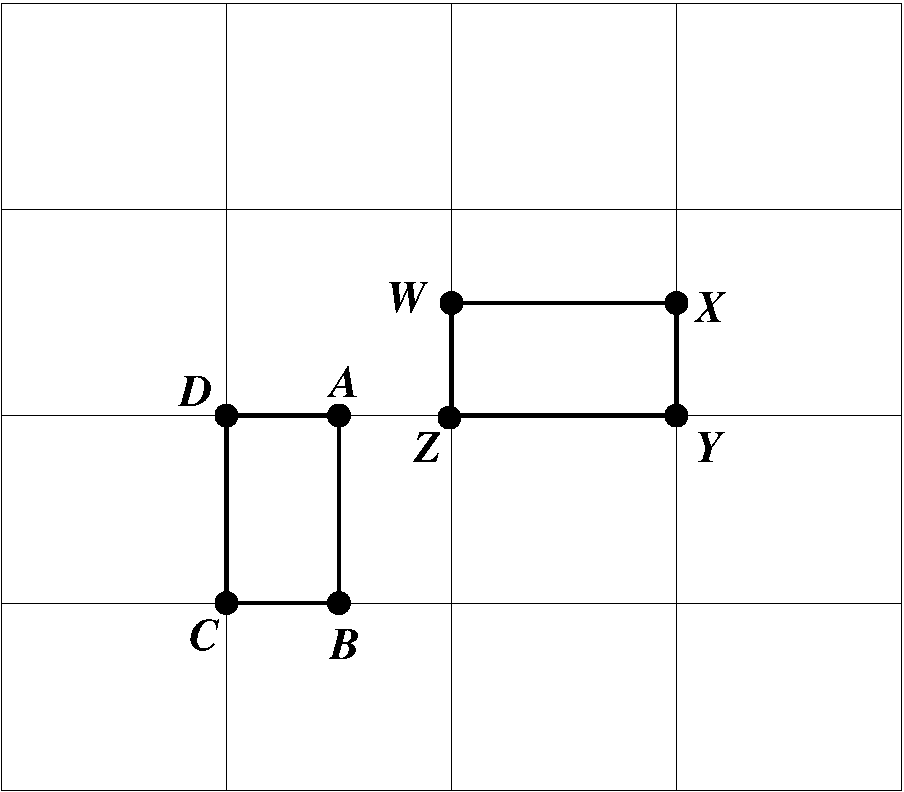
\includegraphics[height=1.3in]{genomics/grid.pdf}
\caption{Example grid.}
\label{fig:grid}
\end{figure}

\begin{figure}
\framebox{\parbox[c]{6.2in}{
$\bullet$ Phase $0$ and $1$ are same as protocol 2.

$\bullet$ {\it [Phase 2] Compute the random shares for values on the grid:}\\ We
compute the random shares for all values on the grid in the row-major
order.  Consider a value $D(i,j)$ on the grid and the rectangle ${\it
rect}(D(i,j,),l,w)$ with $l \; = \; i - k \lfloor \frac{i-1}{k}
\rfloor$ and $w \; = \; j - k \lfloor \frac{j-1}{k} \rfloor$. The reader
can check that all values in the grid ${\it rect}(D(i,j,),l,w)$ lie on
the grid of granularity $k$.  Let $C_{D(i,j)}$ be the circuit for
computing $D(i,j)$ in terms of inputs ${\it bottom}(D(i,j),l,w)$,
${\it left}(D(i,j),l,w)$, $ \alpha [ i-l+1 \cdots  i ]$, and $\beta
[ j-w+1 \cdots j]$.  Note that circuit $C_{D(i,j)}$ can be
constructed by essentially mimicking the proof of
lemma~\ref{lemma:circuit}. Recall that we also have random shares for
the values in the set ${\it bottom}(D(i,j),l,w)$ and ${\it
left}(D(i,j),l,w)$. Now using the protocol for secure computation
shares we can compute the random shares for $D(i,j)$. Essentially this
is similar to phase 2 of Protocol 2 but using $C_{D(i,j)}$ instead of $\CM$. }}
\caption{Protocol 3.}
\label{fig:protocol-3}
\end{figure}
